\documentclass{beamer}

\mode<presentation> {
	\usetheme{Madrid}
}

\usepackage{graphicx}
\usepackage{booktabs}
\usepackage{cite}
\usepackage{tabularx}
\usepackage{csquotes}
\usepackage{subfig}

\graphicspath{{images/}}

\title[Robotics \& Automation]{Evaluating Hierarchical Deep Learning Methods For Vision Based Robot Manipulation Of Dynamic Objects In Unstructured Environments}

\author[CET]{
	Department for Interdisciplinary Research\\ College of Engineering Trivandrum
}

\begin{document}
	
	\begin{frame}
		\maketitle
		
		\begin{tabularx}{\textwidth}{lXl}
			\textbf{Guided by,} & & \textbf{Presented by,} \\
			Linu Shine & & Sreejith Krishnan R \\
			Electronics and Comm. Engg. & & Robotics \& Automation
		\end{tabularx}
	\end{frame}
	
	\section{Motivation}
	
	\begin{frame}
		\frametitle{Motivation}
		Why robot manipulation?
		
		\begin{itemize}
			\item In order to assist in general tasks, autonomous robots should be able to interact with dynamic
			objects in unstructured environments
			
			\item Designing machines that can grasp and manipulate objects with anything approaching human levels of dexterity is first on the to-do list for robotics \cite{graspstate}
		\end{itemize}
		
		Hierarchical reinforcement learning allows to,
		
		\begin{itemize}
			\item Decompose complex task into hierarchy of sub-tasks
			\item Reuse sub-tasks in similar domain
			\item DNA for artificial intelligent agents
		\end{itemize}
	
		\begin{center}
			\textquote[Satinder Singh]{
				Stop learning tasks, start learning skills
			}
		\end{center}
	\end{frame}

	\section{Literature Survey}
	
	\begin{frame}[allowframebreaks]
		\frametitle{Literature survey}
	
		\begin{tabular}{m{2.25cm} | m{9cm}}
			\hline
			
			\textbf{Title} &
			Comparing Task Simplifications to Learn Closed-Loop Object Picking Using Deep Reinforcement Learning \cite{tasksimplification} - IEEE Robotics and Automation Letters - 2019\\
			\hline
			
			\textbf{Methodology} &
			Uses autoencoder to reduce dimensionality of camera data which is given to 3 layer CNN to get a low dimensional encoding. This encoding is used by a 2 layer feed-forward neural network to predict the optimum action. Uses RL to train the mentioned networks\\
			\hline
			
			\textbf{Merits} &
			\begin{itemize}
				\item No hand labeled data required
			\end{itemize} \\
			\hline
			
			\textbf{Demerits} &
			\begin{itemize}
				\item Low success rate (78\%) for manipulation of objects in clutter by real robot
				\item Non modular. Difficult to reuse model for similar task
			\end{itemize}\\
			\hline
			
		\end{tabular}
	
		\begin{tabular}{m{2.25cm} | m{9cm}}
			\hline
			
			\textbf{Title} &
			Regularized Hierarchical Policies for Compositional Transfer in Robotics \cite{rhpo} - DeepMind - 2019\\
			\hline
			
			\textbf{Methodology} &
			Use hierarchical modular policies for continuous control. \\
			\hline
			
			\textbf{Merits} &
			\begin{itemize}
				\item Best sample efficiency on both simulated and real robot
				\item Uses MPO optimization algorithm which reduces the number of hyperparameters
			\end{itemize} \\
			\hline
			
			\textbf{Demerits} &
			\begin{itemize}
				\item High level tasks are not automatically decomposed to sub tasks
				\item Low level policy is shared across all low level tasks making interpretability complicated
				\item Transferring specific skills from sub-tasks policy in a predictable manner is difficult
				\item Experiment results are obtained using model whose inputs include pose of objects in workspace
			\end{itemize}\\
			\hline
			
		\end{tabular}
	\end{frame}
	
	\section{Research Gap and Objectives}
	\begin{frame}
		\frametitle{Research Gap and Objectives}
		\textbf{Research Gap}
		\begin{itemize}
			\item Low success rate when transferring policies from simulation to real world
			\item Low sample efficiency
			\item Low interpretability of learned models
			\item Predictable transfer of learned skills are difficult
			\item Manual task decomposition
		\end{itemize}
		\vspace{1em}
		\textbf{Objective} \\
		Compare RHPO Hierarchical Reinforcement Learning Algorithm for vision based robot manipulation with baseline RL algorithms - PPO and DDPG
	\end{frame}

	\section{Objectives}

	\begin{frame}[allowframebreaks]
		\frametitle{Methodology}
		
		\begin{columns}[c]
			\column{0.45 \textwidth}
			\begin{itemize}
				\item HRL method will be evaluated based on success rate, mean picks per hour and training time
				\item Simulation environment will be created on Bullet Physics Simulator
				\item For fast experiment feedback loop, experiments will be run in distributed fashion. Simulation environments will be tuned for maximum throughput.
			\end{itemize}
			
			\column{0.5 \textwidth}
			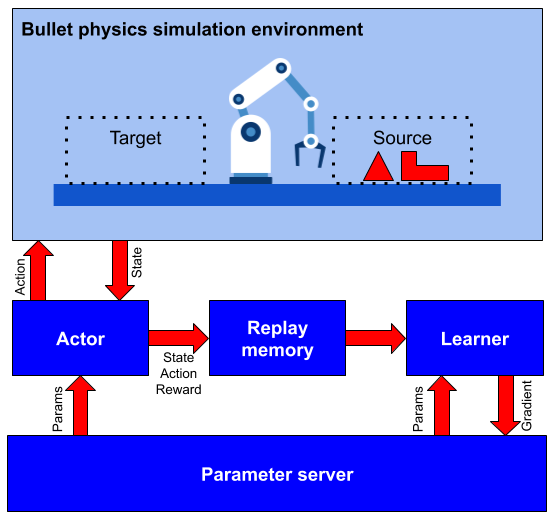
\includegraphics[width=6cm]{setup}
		\end{columns}
	

		\begin{itemize}
			\item HRL algorithm will be compared with baseline model free continuous action space PPO, DDPG and RHPO algorithms
			\item For evaluating transferability of skills, similar tasks like table clearing and stacking of objects will be considered and reduction in training time will be measured
			\item Policies learned from simulator will be evaluated on ABB IRB 120 robot. Depth camera mounted on endeffector will provide visual feedback. Camera will be directly connected to computer. Program running in the computer will directly connect with via serial port in robot controller. RAPID program running on robot will read actions send from computer, execute it and send feedback to computer.
		\end{itemize}
	\end{frame}

	\section{Results}
	\begin{frame}
		\frametitle{Results}
		\framesubtitle{ABB IRB 120 simulator}
		
		\begin{columns}[c]
			\column{0.5 \textwidth}
			\begin{itemize}
				\item PD control tuned for 1mm positioning accuracy which is same as ABB IRB 120 robot positioning accuracy
				\item 20ms mean action time without rendering and 60ms mean action time with rendering
				\item Multiple simulator instances can be run in parallel to scale up agent sampling throughput
				\item Grasp detection and collision detection algorithms
			\end{itemize}
			
			\column{0.5 \textwidth}
			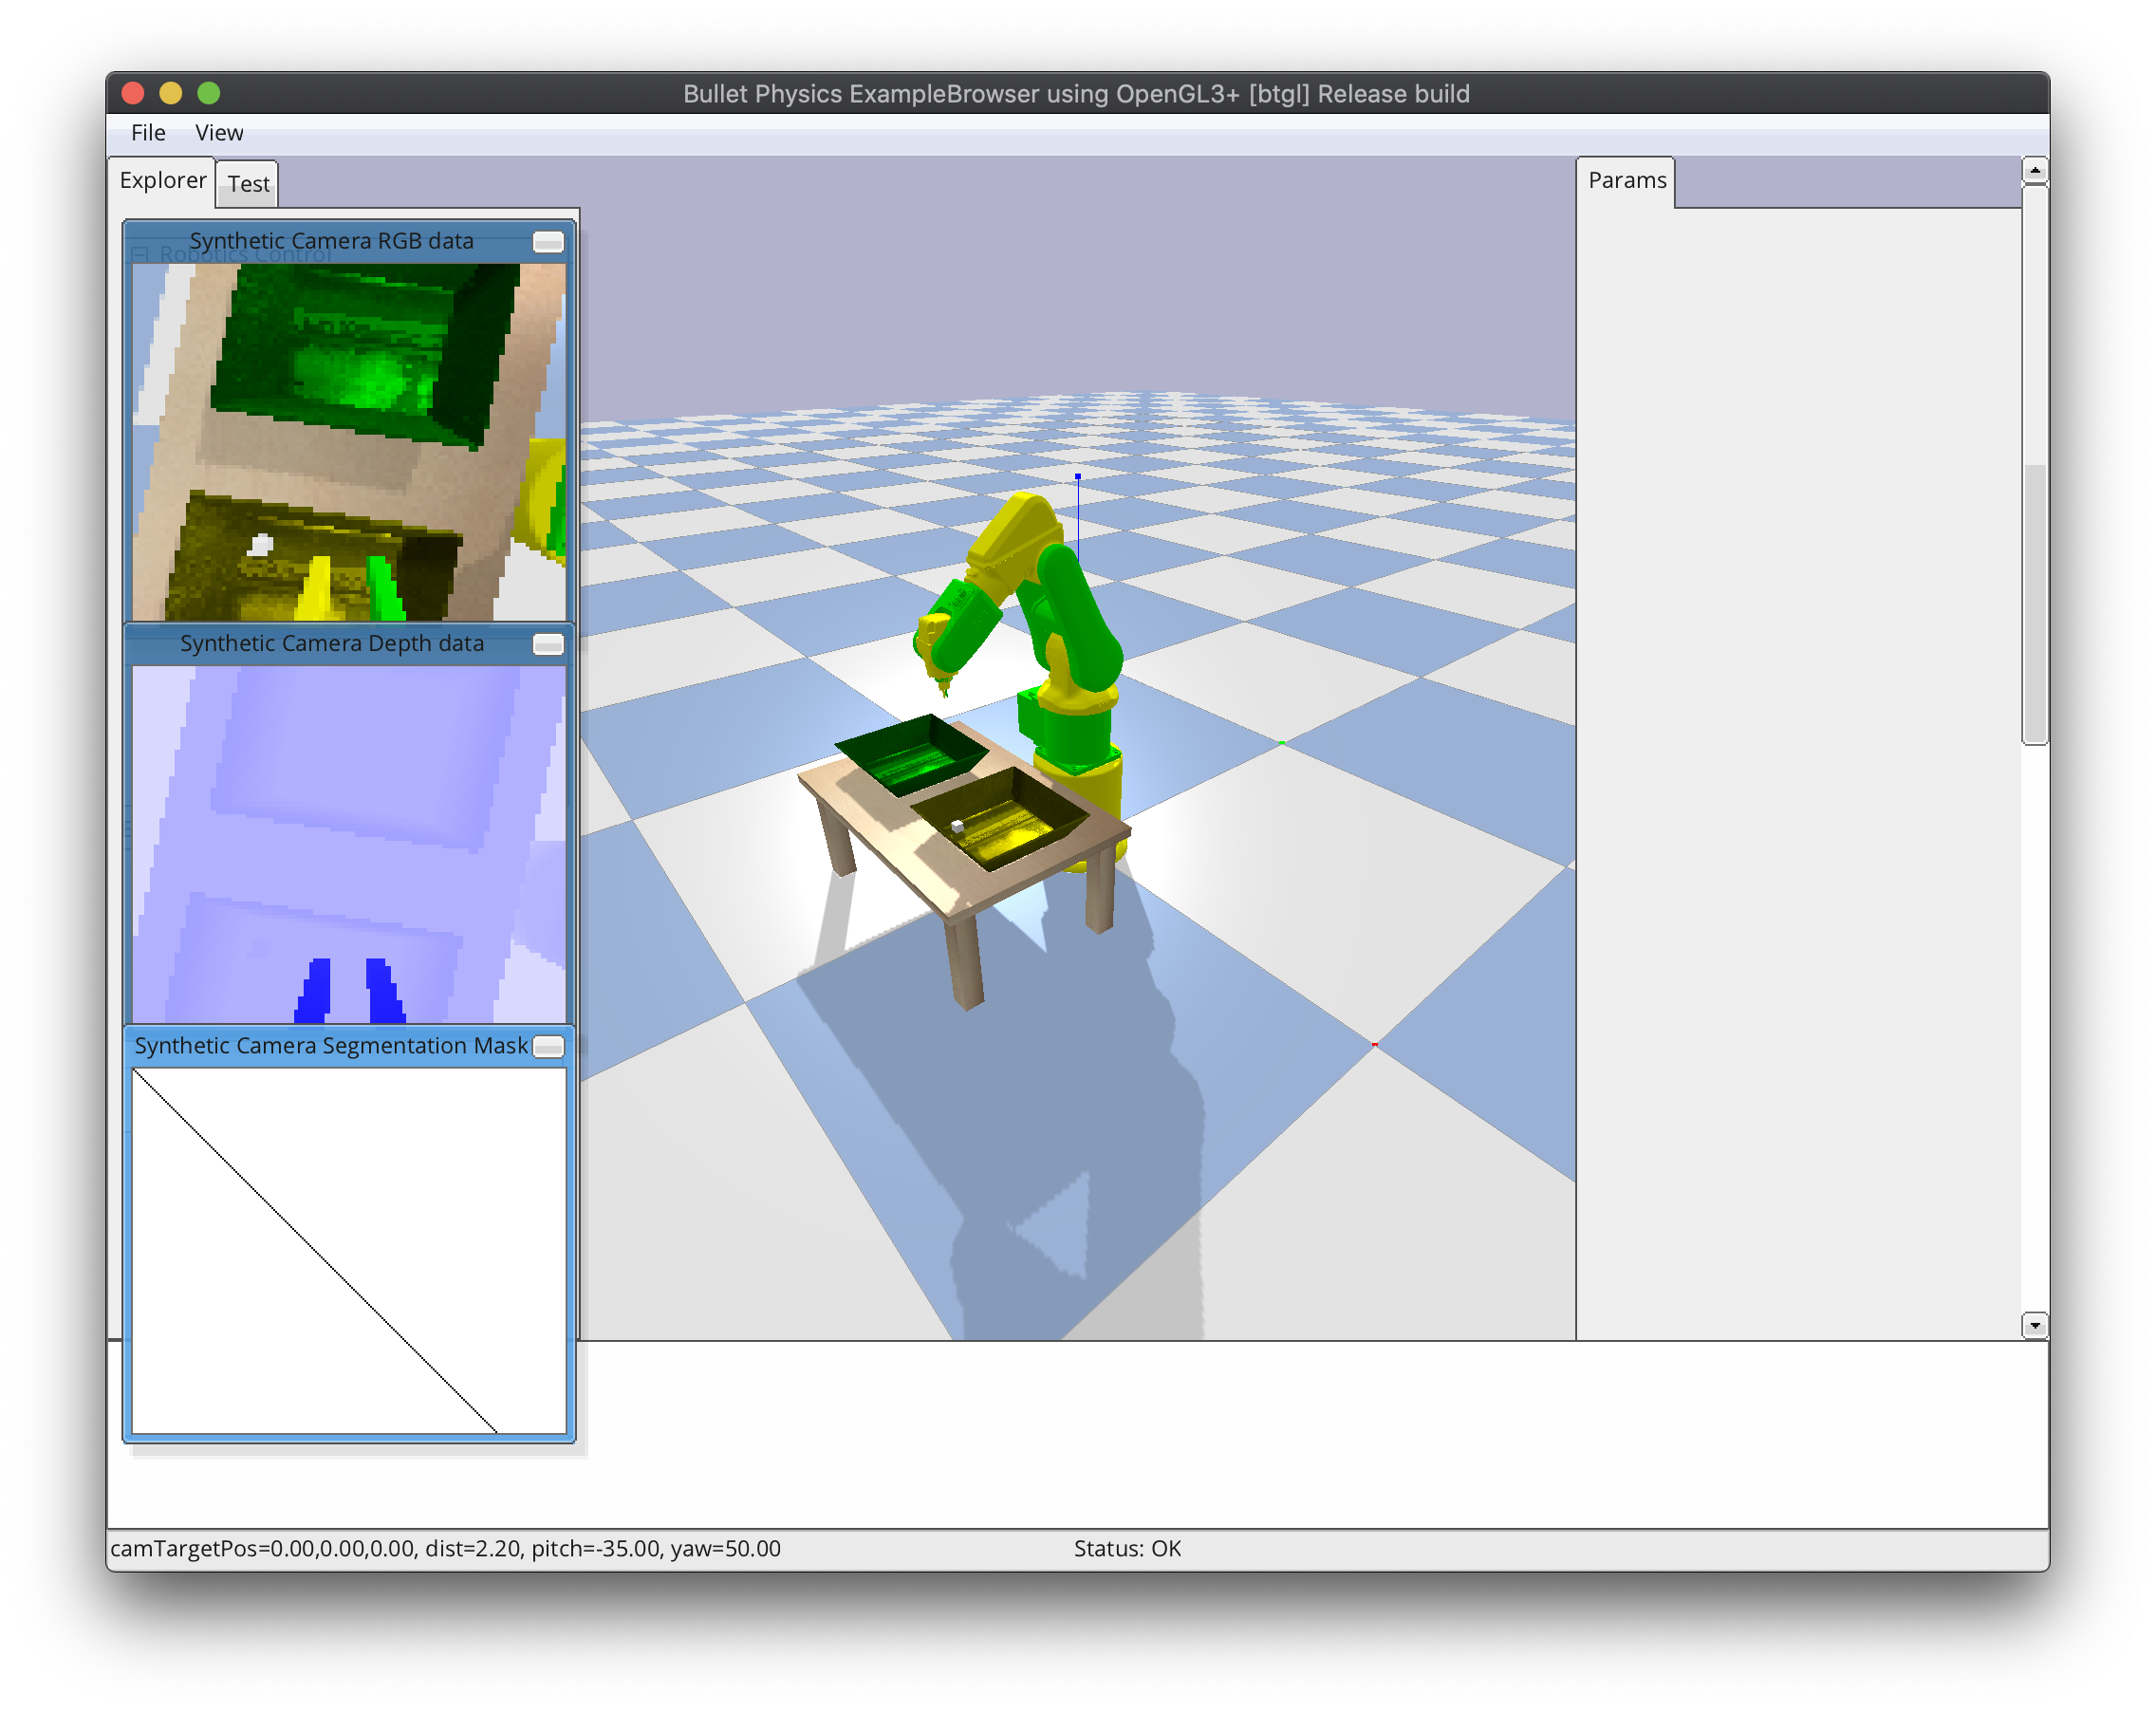
\includegraphics[width=6cm]{simulator.png}
		\end{columns}
	\end{frame}

	\begin{frame}
		\frametitle{Results}
		\framesubtitle{Experiment Setup}
		
		\begin{columns}[c]
			\column{0.5 \textwidth}
			\begin{itemize}
				\item Task is to move the object from yellow tray to green tray
				\item Only input to RL model is the depth image from RGB-D camera mounted on end effector. Observation space is of shape $84x84x4$
				\item RL model can move and rotate the end effector by providing input relative to coordinate frame attached to end effector. Binary variable can be modified to open / close gripper. Action space is $[\delta x, \delta y, \delta z, \delta r_x, open]$
			\end{itemize}
			
			\column{0.5 \textwidth}
			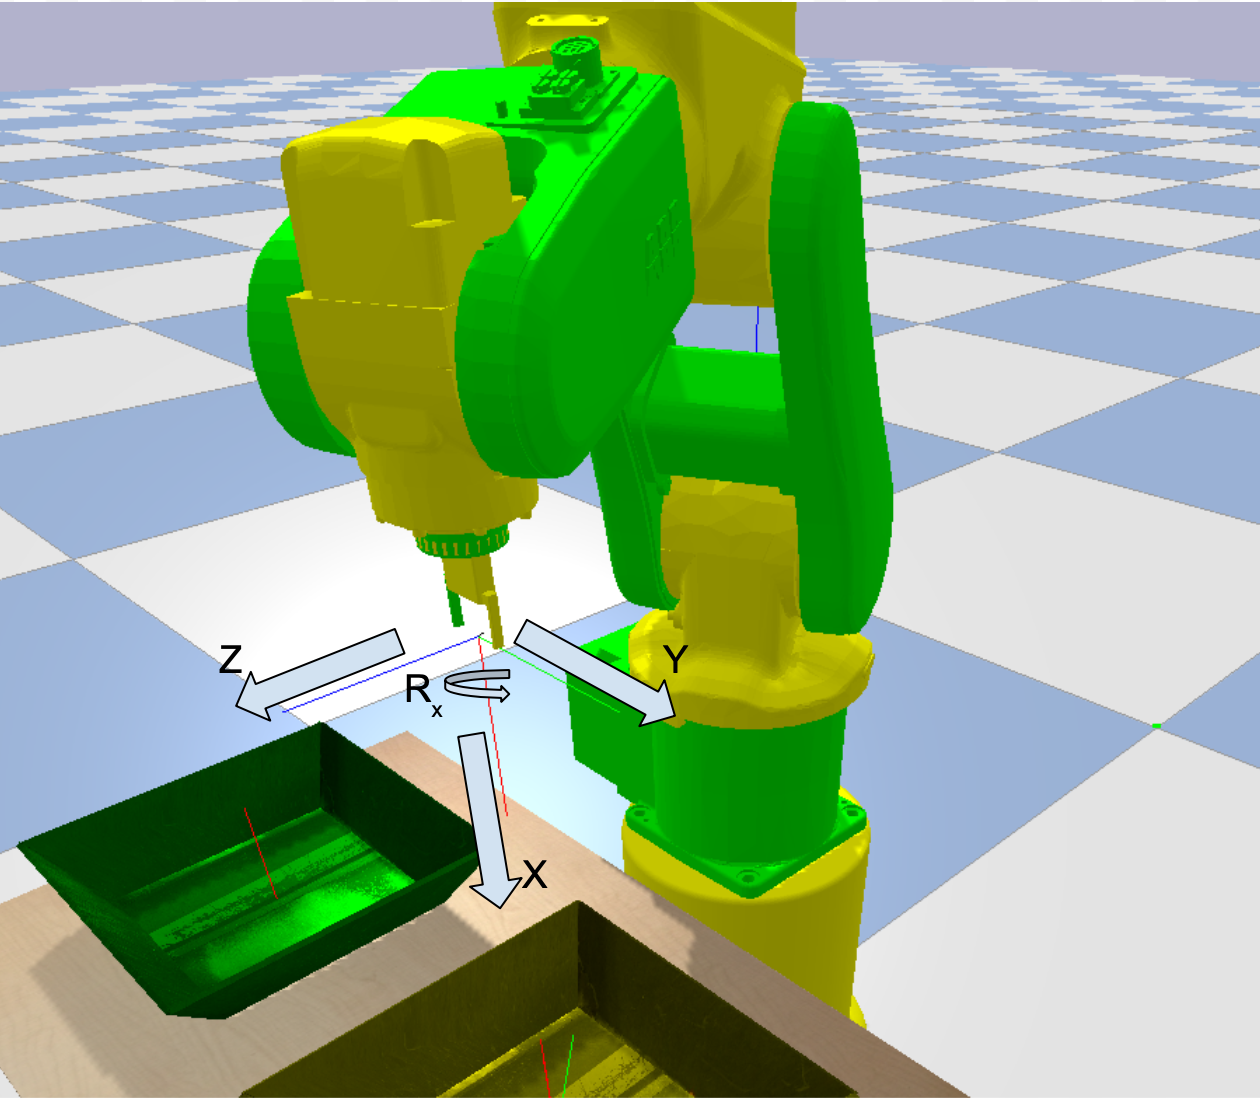
\includegraphics[width=6cm]{action-space.png}
		\end{columns}
	\end{frame}

	\begin{frame}
		\frametitle{Results}
		\framesubtitle{Baseline PPO}
		\begin{columns}[c]
			\column{0.6 \textwidth}
			\begin{itemize}
				\item Convolution layers are used for feature extraction
				\item Input in RGB-D 84x84x4 matrix
				\item Value network predicts the how good it is to be at a particular state
				\item Policy network directly predicts the mean and standard deviation of a Gaussian PDF from which actions are sampled for a particular state
				\item Train batch size is 10240 and SGD minibatch size is 512. Number of iterations per train batch is 30
				\item Data from an episode is added to train batch only after the it is complete
			\end{itemize}
			
			\column{0.4 \textwidth}
			\begin{figure}
				\small{Architecture}
				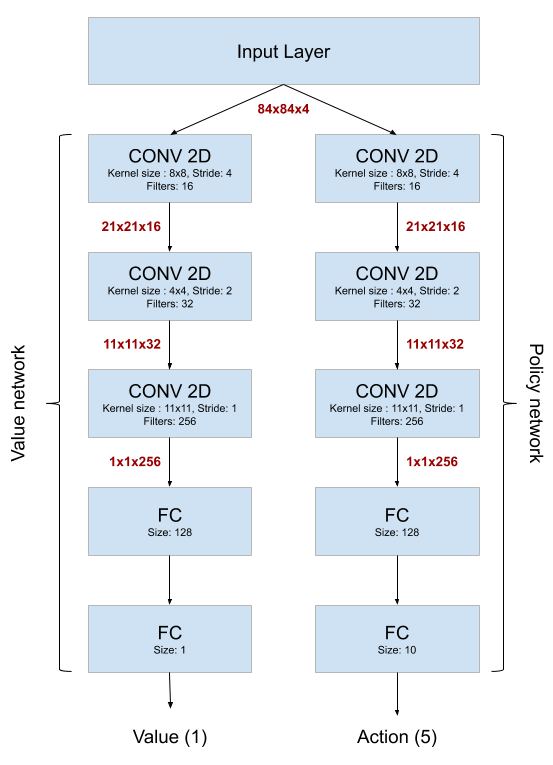
\includegraphics[scale=0.25]{visionnet-arch.png}
			\end{figure}
		\end{columns}
	\end{frame}

	\begin{frame}
		\frametitle{Results}
		\framesubtitle{Baseline PPO}
		\begin{figure}
			\begin{tabular}{cc}
				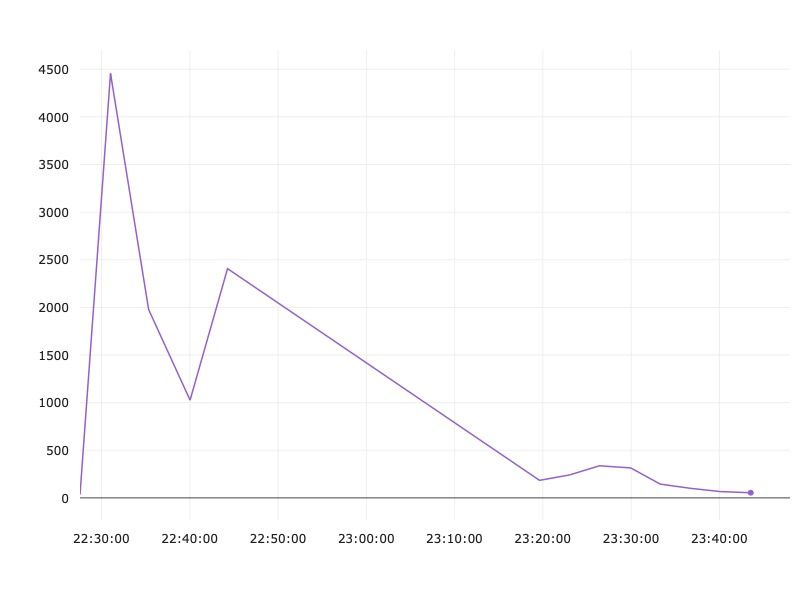
\includegraphics[scale=0.15]{graph-value-loss.jpeg} & 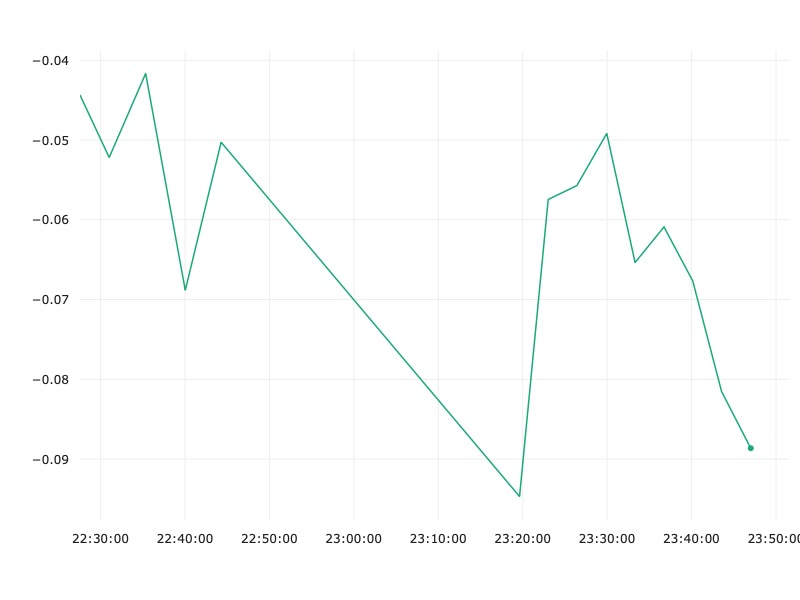
\includegraphics[scale=0.15]{graph-policy-loss.jpeg} \\
				{\small Value network loss} & {\small Policy network loss} \\
				
				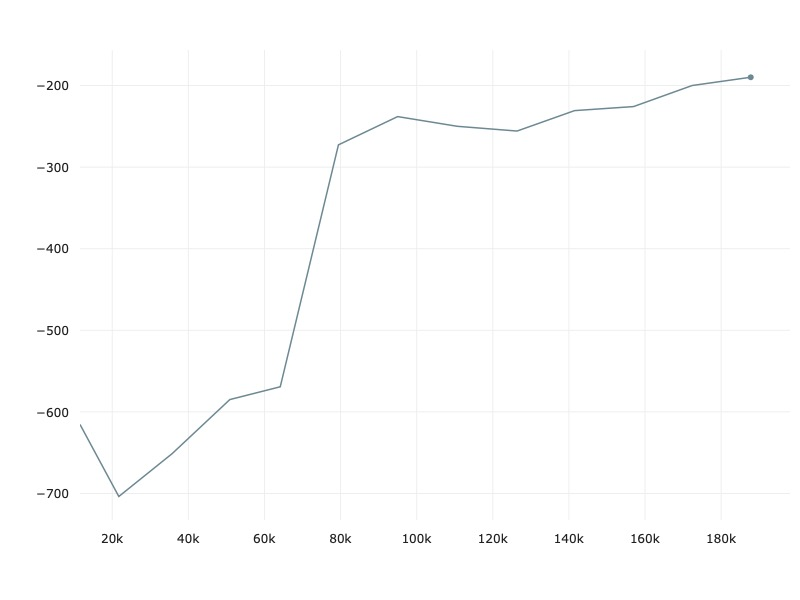
\includegraphics[scale=0.15]{graph-collision-penalty.jpeg} & 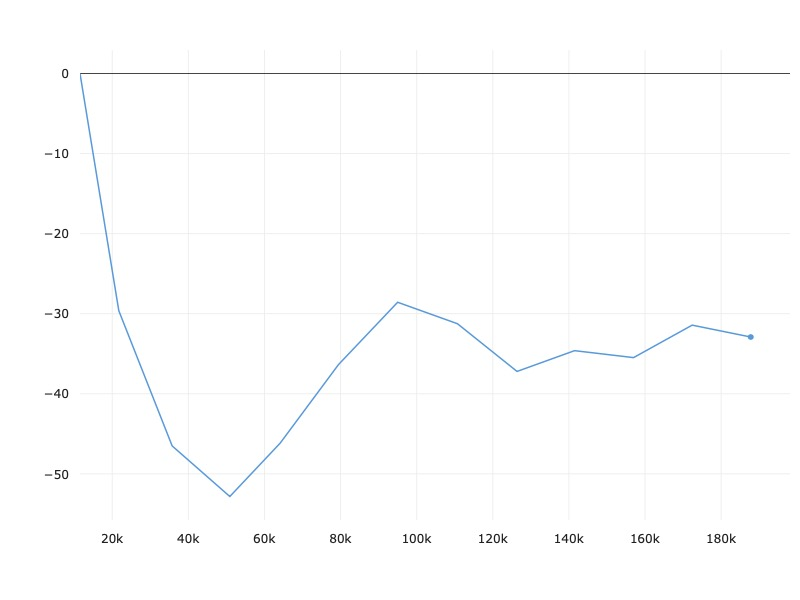
\includegraphics[scale=0.15]{graph-drop-penalty.jpeg} \\
				{\small Collision penalty} & {\small Drop penalty} \\
			\end{tabular}
		\end{figure}
	\end{frame}

	\begin{frame}
		\frametitle{Results}
		\framesubtitle{Baseline PPO}
		\begin{columns}[c]
			\column{0.5 \textwidth}
			\begin{itemize}
				\item Reward shaping is critical. Small changes in reward function can change the learning process.
				\item Providing +ve reward when end effector moves towards target and -ve reward when end effector moves away will not work
				\item Initializing each episode at a random state like grasped and not grasped can improve training speed
			\end{itemize}
			
			\column{0.45 \textwidth}
			\begin{figure}
				\begin{tabular}{c}
					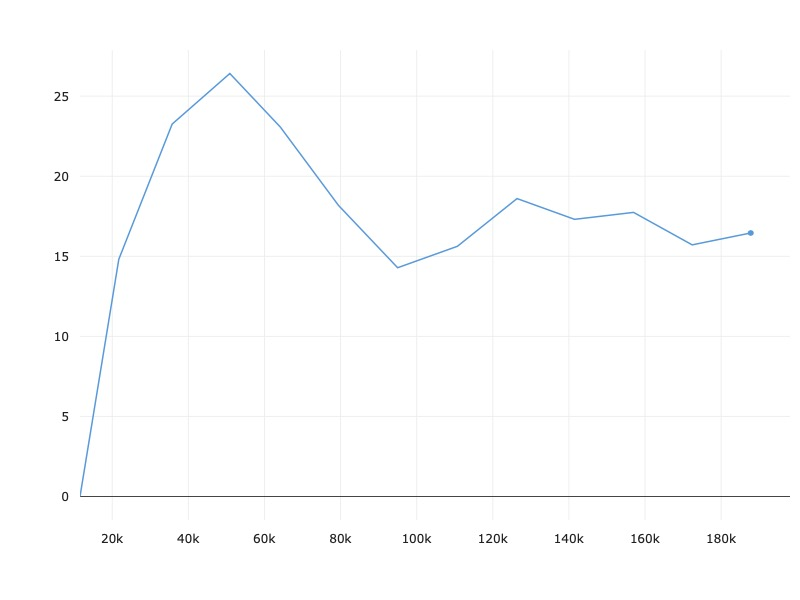
\includegraphics[scale=0.15]{graph-grasp-reward.jpeg} \\
					{\small Grasp Reward} \\ 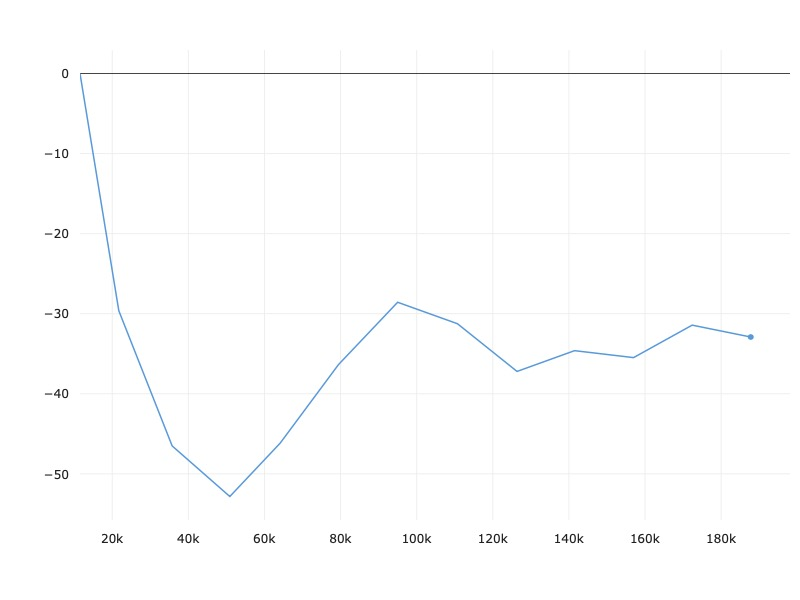
\includegraphics[scale=0.15]{graph-drop-penalty.jpeg} \\
					{\small Drop Penalty} \\
				\end{tabular}
			\end{figure}
		\end{columns}
	\end{frame}

	\section{Future scope}
	\begin{frame}
		\frametitle{Future scope}
		
		\begin{itemize}
			\item Including DDPG and RHPO baseline models
			\item Evaluating baseline models on real robot
			\item Exploring methods for automatic task decomposition
		\end{itemize}
	\end{frame}

	\section{References}
	\begin{frame}
		\frametitle{References}
		
		\bibliography{references}
		\bibliographystyle{unsrt}		
	\end{frame}
	
\end{document} 